% Name: Block on an inclined plane
% Description: A block on a slope at angle θ: its weight, split into parts along and across the slope, the normal force, and friction.
% Tags: inclined plane, forces, components, friction

\usetikzlibrary{arrows.meta, angles, quotes}

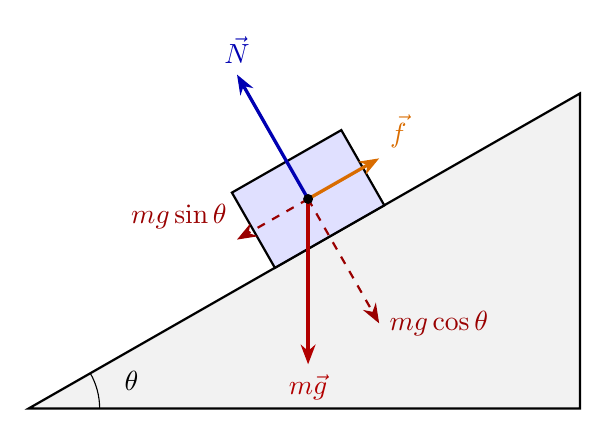
\begin{tikzpicture}[>={Stealth[length=2.5mm]}, force/.style={->, very thick}]
  \coordinate (A) at (0,0);
  \coordinate (B) at (7,0);
  \coordinate (C) at (7,4);
  \draw[thick, fill=gray!10] (A) -- (B) -- (C) -- cycle;
  \pic[draw, "$\theta$", angle eccentricity=1.5, angle radius=9mm] {angle = B--A--C};
  % The slope rises at atan(4/7), about 29.7 degrees; inside this scope x runs up the slope.
  \begin{scope}[rotate around={29.74:(A)}]
    \draw[thick, fill=blue!12] (3.6,0) rectangle (5.2,1.1);
    \coordinate (G) at (4.4,0.55);
    \draw[force, blue!70!black] (G) -- ++(0,1.82) node[above] {$\vec{N}$};
    \draw[force, orange!85!black] (G) -- ++(1.04,0) node[above right] {$\vec{f}$};
    \draw[->, thick, dashed, red!60!black] (G) -- ++(-1.04,0) node[above left] {$mg\sin\theta$};
    \draw[->, thick, dashed, red!60!black] (G) -- ++(0,-1.82) node[right] {$mg\cos\theta$};
  \end{scope}
  \draw[force, red!70!black] (G) -- ++(0,-2.1) node[below] {$m\vec{g}$};
  \fill (G) circle (1.8pt);
\end{tikzpicture}
